% Metódy inžinierskej práce

\documentclass[10pt,slovak,a4paper,twoside]{article}

\usepackage[slovak]{babel}
%\usepackage[T1]{fontenc}
\usepackage[IL2]{fontenc} % lepšia sadzba písmena Ľ než v T1
\usepackage[utf8]{inputenc}
\usepackage{graphicx}
\usepackage{float}
\usepackage{url} % príkaz \url na formátovanie URL
\usepackage{hyperref} % odkazy v texte budú aktívne (pri niektorých triedach dokumentov spôsobuje posun textu)
\usepackage{framed}
\usepackage{cite}
\usepackage{times}

\graphicspath{ {./img/} }

\pagestyle{headings}

\setlength{\parindent}{4ex}

\title{Využitie Natural Language Processing pre lepšie učenie jazyka\thanks{Semestrálny projekt v predmete Metódy inžinierskej práce, ak. rok 2020/21, vedenie: J. Sitarčík}} 

\author{Branislav Hozza\\[2pt]
	{\small Slovenská technická univerzita v Bratislave}\\
	{\small Fakulta informatiky a informačných technológií}\\
	{\small \texttt{xhozza@stuba.sk}}
	}

\date{\small 8. október 2020} 

\begin{document}

\maketitle
%Abstrakt
\begin{abstract}
	V tejto práci sa zameriavame na zlepšenie učenia jazyka pomocou NLP \cite{litman2016natural}. 
	Výhody NLP majú bohaté využitie v učení ako napríklad prístup k obrovskému zdroju textov. 
	NLP sa dnes využíva v mnohých odvetviach či už ako nástroje na rozpoznávanie reči alebo pomocník na opravu gramatických chýb. 
	V edukačnom systéme sa dá hlavne využiť na výučbu jazykov. NLP dokáže vyhodnocovať komplexnosť textu a kontrolovať gramatiku či plagiátorstvo. 
	Tento dokument bude zameraný hlavne na možné využitia a výzvy, ktorým musíme čeliť pri využití NLP technológie. 
	Zameriam sa na to ako NLP učí o jazykoch a ako učí samotný jazyk.
\end{abstract}
%Úvod
\section{Úvod}\label{uvod}
NLP\footnote{Natural Language Processing - spracovanie prirodzeného jazyka} sa v dnešnej dobe používa takmer v každom odvetví, či už v zdravotníctve, 
v informatike, kontrola textu, dátová analýza, atď. S príchodom nových technológií ako sú napríklad \textit{Big Data}, strojové učenie a 
MOOC\footnote{Massive open online course - veľké online kurzy} sa otvorili mnoho možností, ako využiť NLP v praxi. 
V produkcii je už aktuálne mnoho aplikácii, ktoré túto technológiu využívajú pri rôznych kurzoch.
V edukačnom systéme si môžeme ukázať v zozname:
\begin{itemize}
	\item Vyučovanie lingvistických predmetov.
	– napr., čítanie, písanie, rozprávanie
	\item Používanie NLP v potrebách študentov alebo učiteľov
	– napr., knihy, učebné materiály, softvér
	\item Učenie matematiky alebo fyziky
	– napr., vytváranie slovných úloh, generovanie príkladov
\end{itemize}

Táto technológia má veľký potenciál vo využití pri učení anglického jazyka 
alebo STEM\footnote{Science, technology, engineering and mathematics - veda, technológia, inžinierstvo a matematika} predmetoch. 
Pri tejto forme štúdia vieme NLP využiť na kontrolu gramatiky pri písaní esejí, učenie slovíčok alebo správnej výslovnosti.
Ako najväčšiu výhodu využitia tejto technológie v praxi vidíme hodnotenie testov s veľkým počtom testovaných študentov. 
Okrem korektnosti testov sme schopní taktiež kontrolovať plagiátorstvo textu.

Ako môžeme vidieť v obrázku Č.\ref{nlp_obrazok}, výskum v aplikovaní NLP v edukačnom systéme spočíva v opakujúcom sa cykle. 
Technologické inovácie sú inšpirované sociálnymi potrebami. Technologický výskum je najprv informovaný a následne prispieva 
do edukačnej teórie a poskytuje dáta.

V časti \ref{NLP} si vysvetlíme v skratke čo je NLP, v časti \ref{ucenie_o_jazyku} sa pozrieme na učenie o jazyku pomocou NLP, 
v časti \ref{ucenie_pomocou_nlp} vysvetlíme ako sa využíva NLP pri učení jazyka a v časti \ref{spracovanie_jazyka} zisťujeme ako 
spracovanie jazyka pomocou NLP pomáha ľudom lepšie učiť a ďalej skúmať NLP.
\begin{framed}
\begin{figure}[H]\label{nlp_obrazok}
	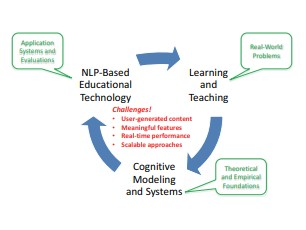
\includegraphics[width=0.9\textwidth]{nlp}
	\centering
	\caption{Cyklus technologickej inovácie}
\end{figure}
\end{framed}1
%Čast o NLP
\section{Natural Language Processing} \label{NLP}
Je to druh umelej inteligencie, zameranej na prácu s textom a obrázkami.  
Táto technológia je spojením lingvistiky a informatiky, 
pričom vzniká snaha aby stroj porozumel prirodzenej reči človeka.
NLP má za sebou 70 rokov vývoja a prvé zmienky sú z roku 1950\cite{historia}.
\subsection{História}
	Už v roku 1950, Alan Turing publikoval článok "Computing Machinery and Intelligence"\cite{turing2009computing} 
	ktorý priniesol tzv. Turingov test ako kritérium inteligencie, pre automaticky generovanú 
	prirodzenú reč. V tej dobe sa NLP nerozlišovalo od umelej inteligencie.\linebreak
	Okolo roku 2010 sa začali rozširovať metódy strojového učenia ako napríklad hlboké učenie alebo 
	\textit{representation learning} aj v NLP, pretože bolo dokázané že tieto techniky sú veľmi účinné.
\subsection{Využitie}
Zoznam možných využití NLP v praxi:
\begin{itemize}
	\item OCR - Optické rozoznávanie znakov
	\item Rozpoznávanie hlasu
	\item Rozklad zvuku na text
	\item Prevod textu na hovorenú reč
	\item Rozklad textu to logických celkov
	\item Morfologická analýza
	\item Syntaktická analýza
\end{itemize}
\section{Využitie NLP pri výučbe jazyka}\label{vyuzitie_jazyka_nlp}
%Čast o učení jazyka
\subsection{Učenie o jazyku} \label{ucenie_o_jazyku}
		Jedným z najstarších a napriek tomu najaktívnejším využití NLP je jeho využitie pri učení jazyka.
	Tento proces zvyčajne pozostáva vo vyhodnotení zručnosti študenta v písaní testov, v čítaní alebo
	rozprávaní v danom jazyku. Syntaktická analýza sa používa na detekciu a potenciálne opravenie chybného použitia
	predložiek pri skupinách ako sú ESL\footnote{English as second language - ľudia pre ktorých angličtina nie je primárny jazyk.} alebo hluchý študenti.

	Aktuálne potreby pri vymýšľaní testov a výučbových lekcií posúvajú tento odbor vopred niekoľkými smermi. Môžeme sa na to pozrieť z viacerých hľadísk. 
	Z hľadiska textu ako napríklad vytváranie testov, písomných úloh a ústne skúšanie sa rozvíjajú a prinášajú nové výzvy pre existujúce metódy výučby.
	Ako príklad si môžeme uviesť automatické vyhodnocovanie písomných testov pri MOOC, ktoré je pre MOOC kľúčové. Tento proces pomohol rozšíriť výskum analýzy textu, 
	ktorý bol generovaný počas štandardizovaného textu využitého v teste. Okrem toho niektoré MOOC používajú dobrovoľníkov na vyhodnocovanie testov, 
	kvôli slabej spoľahlivosti alebo presnosti systému. Namiesto toho by radšej mohli plne automatizovať vyhodnocovacie metódy.
%Čast o učení pomocou NLP
\subsection{Učenie jazyka} \label{ucenie_pomocou_nlp}
	Narozdiel od využitia ako analýzy (viď. predošlá časť), jazyk môže byť využitý aj ako výučbová metóda.
	V článku z roku 2011\cite{clanok_o_studovani} bolo dokázané, že skupina detí ktoré sa učia pomocou živého učiteľa, 
	pochopili látku lepšie ako žiaci, ktorí sa učili pomocou PC. Hlavným rozdielom medzi ľudským učiteľom a PC učiteľom 
	je, že iba človek vie používať prirodzené vety.

	V posledných rokoch sa systémy založené na dialógu snažia výkonovo čo najviac priblížiť prirodzenej ľudskej reči. 
	Uvažovalo sa aj nad tým, že učenie by sa malo odohrávať vo viac sociálno realistickom prostredí aby sa \textit{PC učiteľ} vedel viac adaptovať študentom.
%Čast o spracovaní jazyka
\subsection{Spracovanie jazyka} \label{spracovanie_jazyka}
	Okrem úlohy NLP ako prostriedok na spracovanie textu a hovorenej reči pri vyhodnocovaní testov, 
	alebo ako médium medzi učivom a výkladom, má NLP aj veľké využitie pri spracovaní textu pre vedcov, 
	učiteľov alebo vývojárov týchto automatizovaných systémov. Využíva sa obrovské množstvo textov a zvukových
	stôp, ktoré sú dostupné v elektronickej podobe na sociálnych sieťach, fórach, blogoch alebo stránkach ako 
	napríklad Wikipédia. Jedným z najväčších zdrojov je tzv. Linguistic Data Consortium\footnote{Linguistic Data Consortium (http://www.ldc.upenn.edu/)}
	
	Ak sa zameriame na výhody spracovania jazyka pre učiteľov, tak sa NLP využíva hlavne na automatizáciu ktoré by boli robené manuálne, 
	ako napríklad: vytváranie učiva alebo pripravovanie testov. NLP môže byť využité aby bolo učivo presne zamerané na základe 
	poskytnutých materiálov z elektronických zdrojov. Výsledkom by mohli byť weby, ktoré by boli žiakom ľahšie pochopiteľné ako odborné články\cite{miltsakaki2009matching}.

\section{Záver} \label{zaver} % prípadne iný variant názvu
	Tento článok bol zameraný na výskum vo využití NLP pri výučbe anglického jazyka. Tento článok bol motivovaný 
	potrebami učiteľov a ľudmi ktorí sa radi učia jazyky. Aj napriek tomu že využitie NLP na učenie je jedno z najstarších využití, 
	nové fenomény ako MOOC a \textit{Big Data} priniesli mnoho nových možností v tomto odvetví a taktiež upevnilo puto medzi výskumom NLP a inými 
	odvetviami umelej inteligencie.

	Tento článok začal analýzou NLP v edukačnom systéme ako takom a následne sme sa zamerali na spôsob využitia pri učení jazyka, 
	učení pomocou jazyka a spracovanie jazyka. V prvej časti sme našli veľký potenciál NLP pri vyhodnocovaní testov, textov a pri skúšaní.
	V druhej časti sme sa pozreli na učení pomocou jazyka, kde sa ale prekážalo že zatiaľ je študentom ľahšie študovať pomocou živého človeka, 
	pretože jeho reč je prirodzenejšia. V poslednej časti sme zistili že NLP dokáže spracovať jazyk z rôznych zdrojov a tak poskytnúť prehľadnejšie dáta
	učiteľom, žiakom ale aj výskumníkom v tejto oblasti. Objavili sme mnohé príležitosti ale aj výzvy, ktorým musíme ešte čeliť.

\bibliography{literatura}
\bibliographystyle{plain} 
\end{document}
